\chapter{Model}
\label{chap:model}

We can understand the specifics of demodularization by describing it as an algorithm for a simple language with a well defined semantics.

\section{A Module Language}
The \emph{mod} language (Figure~\ref{fig:source-lang}) contains only the features necessary to write modular programs where it is possible to observe the effects of module evaluation order.

\begin{figure}[h]
\centering
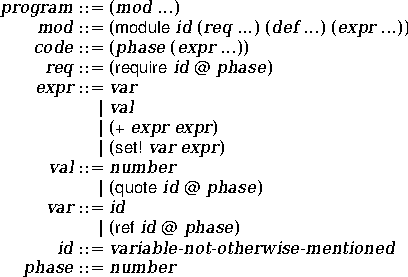
\includegraphics{figures/source}
\caption{\emph{mod} language grammar}
\label{fig:source-lang}
\end{figure}

A program in \emph{mod} consists of a list of modules that can refer to each other.
Each module has a name, any number of imports, any number of definitions, and sequenced code expressions. 
All definitions in a module are exposed as exports to other modules, but to use definitions from another module, the program must import it through a \racket{require} expression.
Both \racket{require} and \racket{define} expressions have phase annotations; this simulates the interactions between modules in a language with macros and a language tower without requiring a model of macro expansion.
The language includes variable references, numbers, addition, and mutation.
Mutation makes module evaluation order observable, and addition represents the work that a module does.
In addition to numbers and variables, there are two special forms of values and references that model the interaction of macros with the module system.
A \racket{quote} expression is like a reference to syntax at runtime.
A \racket{ref} expression is like a macro that can only do one thing: refer to a variable at a phase.

\section{Compilation}

We have to compile \emph{mod} programs before demodularizing them, just like in the Racket implementation.
In Racket, compiling expands all macros in a program and changes definitions and variable references to refer to memory locations.
In \emph{mod}, compiling eliminates \racket{ref} expressions, turns definitions into \racket{set!} expressions, changes variable references to include module information, and sorts code into phases.
Compilation in both cases still leaves behind a relatively high-level language, but the language is free of syntactic extensions.
This is important for demodularization because otherwise macro expansion would have to be part of the algorithm, which would complicate it and possibly duplicate work.
The grammar in Figure~\ref{fig:compiled-lang} specifies the compiled language for \emph{mod}.

\begin{figure}[h]
\centering
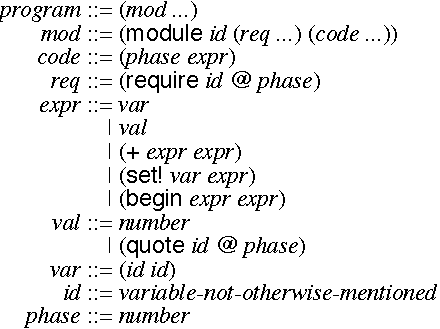
\includegraphics{figures/compiled-lang}
\caption{Compiled language grammar}
\label{fig:compiled-lang}
\end{figure}

The grammar no longer has definitions, all variables now include module references, and code is sorted into phases.
The actual compilation function is not relevant to demodularization.

\section{Evaluation}

We evaluate the compiled language using a small-step reduction semantics. 
Because the reduction rules are syntactic, we extend the compiled language further with evaluation contexts, a heap representation, and a stack representation to keep track of the order to instantiate modules.
These extensions are in Figure~\ref{fig:compiled-eval-lang}.
An expression of the form:
\[
  (\sigma\ /\ program\ /\ ((id\ phase)\ \ldots)\ /\ ((id\ phase)\ \ldots))
\]
represents the state of the machine during evaluation.
$\sigma$ represents the heap of the program, and when evaluation finishes represents the output of the program.
The list of modules is the code of program in the compiled language.
The first list of \racket{(id phase)} pairs is the list of modules to evaluate, and the second list is the modules that have already been evaluated.

\begin{figure}[h]
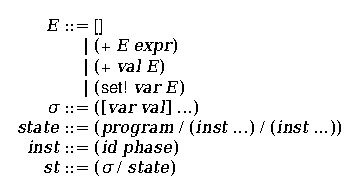
\includegraphics{figures/compiled-eval-lang}
\caption{Extensions to compiled language grammar}
\label{fig:compiled-eval-lang}
\end{figure}

The reduction rules in Figure~\ref{fig:eval-reduction} evaluate a compiled program that starts with an empty heap, the program code, a stack that contains the identifier of the main module at phase 0, and an empty completed module list. 

% TODO: re-render without red
% TODO: maybe needs a rewrite to capture meaning better (Jay's example)
\begin{figure}[h]
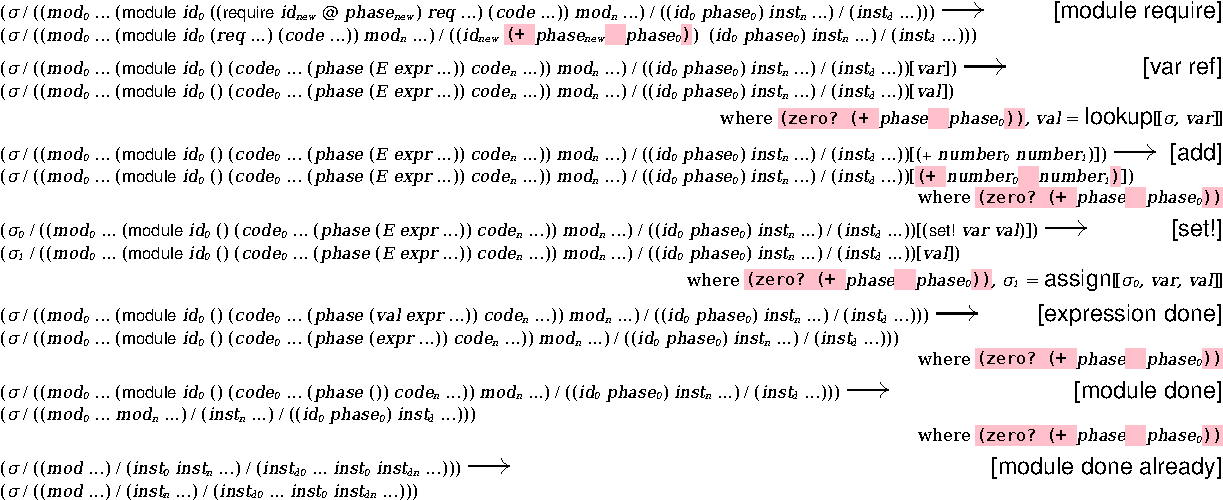
\includegraphics[width=\textwidth]{figures/eval-reduction}
\caption{Modular evaluation}
\label{fig:eval-reduction}
\end{figure}

% TODO: explain that phases are relative
The \emph{module require} rule matches a program with a \racket{require} expression in the module at the top of the evaluation stack and evaluates it by removing the \racket{require} expression from the module and pushing the required module onto the evaluation stack with the phase shifted appropriately.
The current module is still on the stack and will continue evaluating after the required module is done evaluating.
The subsequent rules all apply only when the phase relative to the main module is zero.
The \emph{var ref} rule looks up a variable in the heap and replaces the variable with its current value.
The \emph{add} rule replaces an addition expression of numbers with the result of computing their sum.
The \emph{set!} rule installs a value for a variable into the heap and reduces to the value.
When an expression is a value, the \emph{expression done} rule matches and removes the expression from the module.
When there are no more expressions left in a module, the \emph{module done} rule applies by removing the module from the program and placing a reference to it in the list of finished modules.
The \emph{module done already} rule applies when the current module on the stack is in the finished list, so that modules are not evaluated multiple times. 

\section{Demodularization}

Figure~\ref{fig:demod-redex} shows the demodularization algorithm for the compiled language.

\begin{figure}[h]
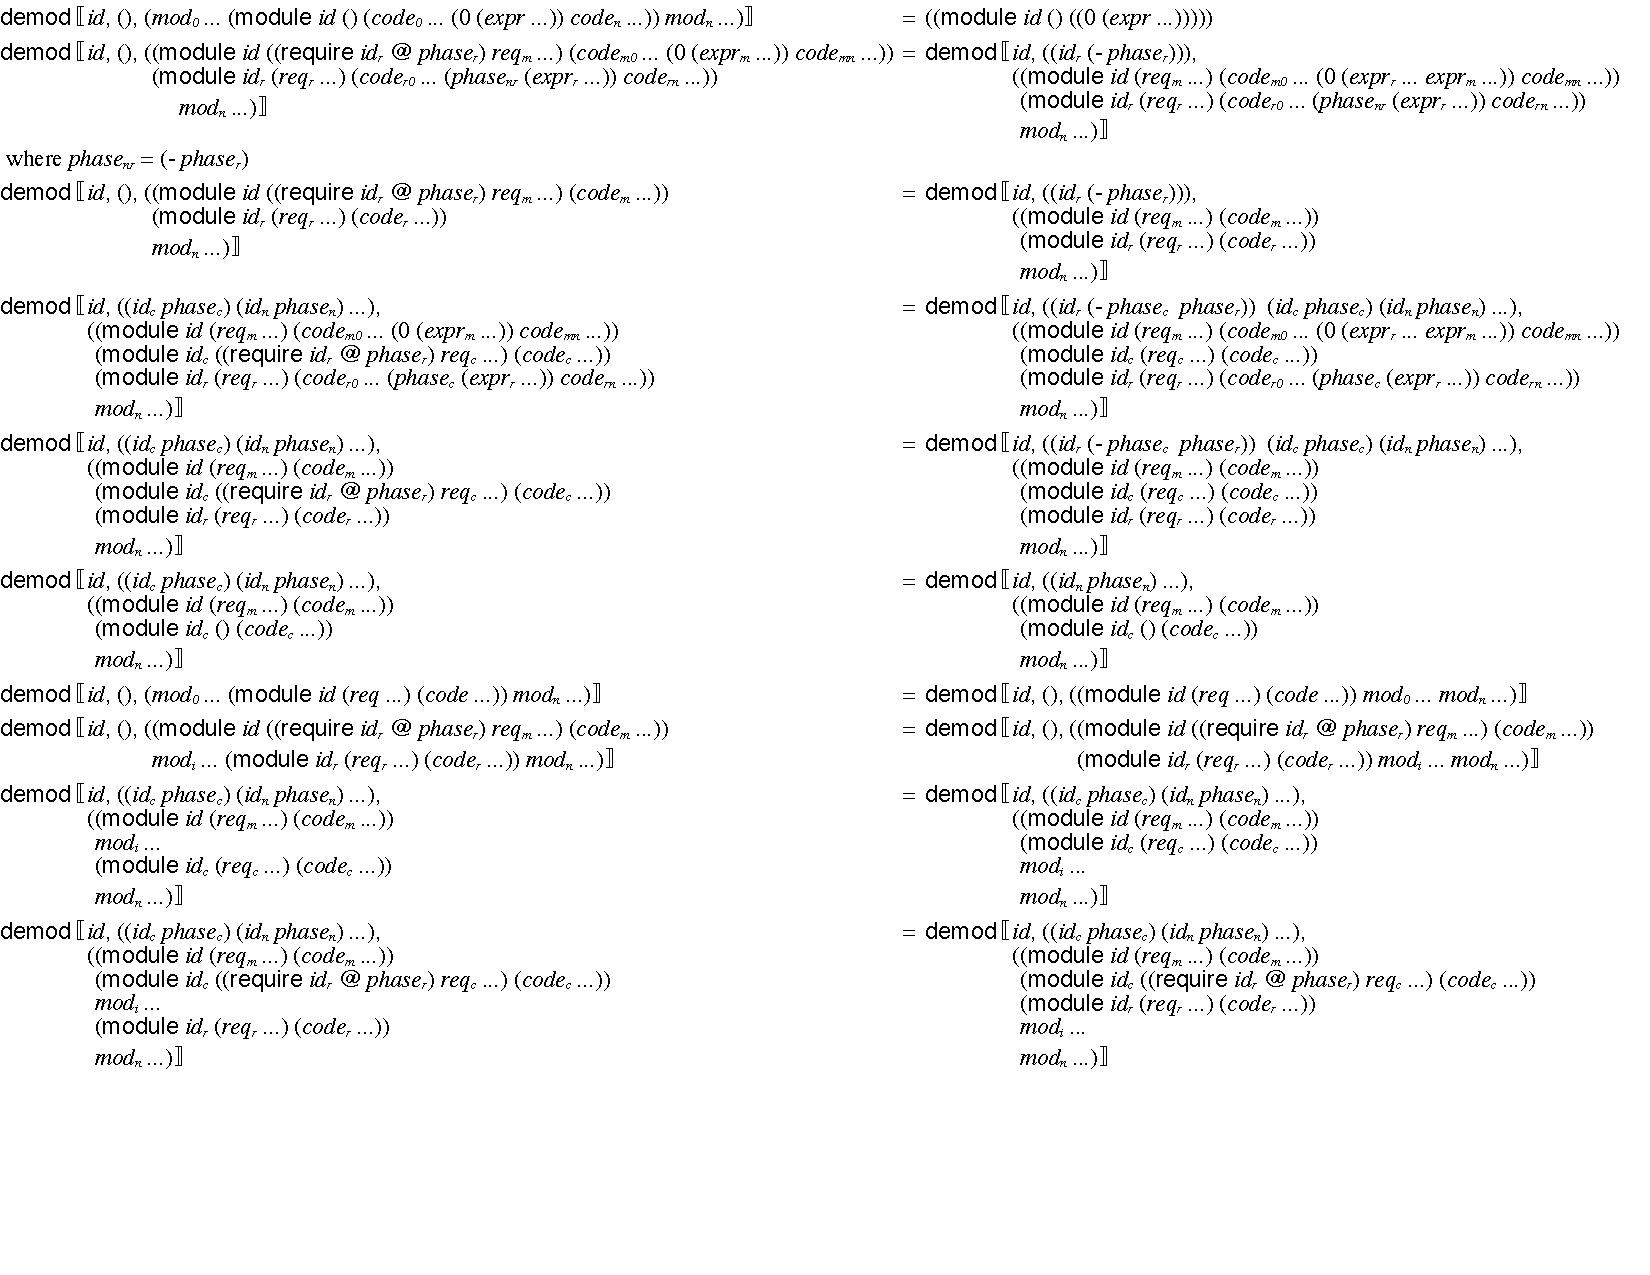
\includegraphics[width=\textwidth]{figures/demod-redex}
\caption{Demodularization algorithm}
\label{fig:demod-redex}
\end{figure}

The algorithm takes as input an \emph{id} specifying the main module of the program, a working list of phased requires, and a list of modules that make up the program.
The first rule applies when the main module has no requires left and there are no requires in the working list, meaning the algorithm can terminate with just the phase 0 code of the main module remaining.

The second and third rules apply when the main module requires the next module in the module list.
Both rules add the required module's \emph{id} to the working list of required modules so that the algorithm will follow the complete require graph.
% TODO: check to see if there is a diamond pattern, will the algorithm handle it correctly (I don't think it will right now)
The second rule handles the case where the required module has code that will be at phase 0 for the main module and puts that code before the existing phase 0 code of the main module.

The next three rules apply when handling the working list of required modules. 
The first of the three is similar to the second rule because it extracts code that will be in phase 0 of the main module and inserts it into the main module.
The second rule of the three working list rules handles the case where there is no matching code for phase 0.
The third rule removes an entry from the working list when the module has no more requires.

The final four rules rearrange the program's module list so that modules that require each other are adjacent in the list and the other rules can apply.

\section{Equivalence}
% TODO: state an actual property and give a proof sketch
We claim that the programs will evaluate to the same answers before and after demodularization. 
This is because the demodularization algorithm is a type of partial program evaluation, doing the same work that the evaluator does but before the program is run.
Specifically, the demodularizer makes it so the \emph{module require} rule of the evaluator never applies because all requires have been inlined.

